\documentclass{article}
\usepackage[utf8]{inputenc}
\title{Lesson 6 - Discrete Mathematics}
\author{Matt Chung}
\date{August 21 2017}
\usepackage{tikz}
\usepackage{verbatim}
\usetikzlibrary{calc}
\renewcommand{\thesubsection}{\thesection.\alph{subsection}}

\begin{document}
\maketitle

\section{}

\subsection{}

\textbf{Solution:} This relation is an equivalence relation.

This relation satisfies the three properties that an equivalence relation exhibits.  First, the relation is reflexive since every person has the same height as themselves. Second, it is symmetric since if $a$ and $b$ have the same height, so does $b$ and $a$. Finally, if $a$ and $b$ have the same height, and $b$ and $c$ have the same height, so do $a$ and $c$. Therefore, this relation is classified as an equivalence relation.

The equivalence class contains everyone who is the same height. For example, the equivalence class of someone who is 5 foot 8 inches contains everyone who stands 5 foot 8 inches tall (or short).

\subsection{}

\textbf{Solution:} This is \textbf{not} an equivalence relation.

This relation only satisfies 2 out of 3 of properties required to be classified as an equivalence relation. The two properties that it exhibits are: reflexive and symmetric. This relation is reflexive because a person shares the same grandparent as themselves; in addition, symmetric because if $a$ and $b$ share the same grandparent, so does $b$ and $a$. However, where the equivalence relation falls apart is the transitive property. For example, imagine Joe and Chris, cousins, share a common grandparent; this link is bonded by their mothers, whom are sisters.  Chris has a cousin, Lisa, on his father's side (i.e. Chris's father has a brother who has a daughter), the two of them sharing a grandfather. This grandfather, however, is not shared with Joe. In other words, Joe and Lisa do not share a common grandfather. Therefore, since this relation does not exhibit the transitive property, it is not considered as an equivalence relation.


\section{}

This is not an equivalence relation. First, it is not reflexive: a person cannot be a brother to themselves. On the other hand, symmetry is satisfied; if $a$ is a brother to $b$, then $b$ is a brother to $a$. Where things get tricky is the third property: transitive. My knee jerk reaction was ``of course the relationship is transitive.'' But that's not true. It's easy to leap to the conclusion if in your frame of mind you only consider three, separate entities: x and y and z. It's easy to picture the transitive relation here; but this does not hold true if we only consider two individuals—x and y. With only two individuals, you would get ``x is a brother y'' (true)  and ``y is a brother of x``, also true; but ``x is a brother of x'' would not be true, for the same reason why the reflexive property failed. 

\section{}

\textbf{Solution:} 4

I had to re-read this question several times, asking myself: what is this question really asking? But I now have a firm grip of what it's asking: what is the least number of elements in the set, while maintaining an equivalence relation. So, we're given the following set: $({a,b,c,d})$. What is the minimum number elements needed to create an equivalent relation? Well, keeping in mind we need to maintain the three properties—reflexive, symmetric, transitive—we would need to construct the following:

${(a,a), (b,b), (c,c), (d,d)}$

\section{}

\subsection{}

A is the set of all ordered pair of positive integers. We define a relation: $(a,b)R(c,d)$ if  $ad = bc$. Now, I need to prove that $R$ is an equivalence relation on A.


Let's step through each property, one by one:

\begin{itemize}

    \item \textbf{reflexive} - Let's start with an example. Say $a$ is 2.  We would get $(2,2)R(2,2)$. In other words, we'd get: $(2)(2) = (2)(2)$. This is true; therefore, this relation is reflexive.
    
    \item \textbf{symmetric} - In another example, let's say we are given $(3,6)R(4,8)$. This relation turned into the mathematical expression is: $(3)(8) = (6)(4)$. Now if we take this relation and flip our set, testing for symmetry, we get the following: $(4,8)R(3,6)$; $(4)(6) = (8)(3)$. Yes, this is true and the relation does satisfy the symmetric property. 
    \item \textbf{transitive} - This is true as well. Piggybacking on the last example, assuming $a$ and $b$ are $(3,6)$ and $(4,8)$, respectively, let's add the another item (i.e. $c$), $(2,4)$, into the mix: $(4,8)R(2,4)$. Does $a$ and $c$ hold true? Let's put it to the test: $(3,6)R(2,4)$. Substituting the set with the equation, we get $(3)(4) = (6)(2)$. This proves that the relation is transitive.
    
\end{itemize}

\subsection{}

Let's assume that each item in the equivalence class $(1,2)$ takes the form $(a,b)$. For each item this set, the value of $b$ is double of $a$. In other words, $a$ is half the valeu of $b$. For example, $(1,2)R(5,10)$. This satisfies the relationship because $(1)(10) = (2)(5)$; once again, another element in this set would be $(3,6)$; we get $(1,2)R(3,6)$, which equals $(1)(6) = (3)(2)$. Effectively, if the element is described as $(a,b)$ in the equivalent class, then we would get $2b = a$.

\section{}

We are given $\{1,2,3,4,5,6\}$. Here are the equivalence classes:
\begin{itemize}
\item $\{1,2,4\}$
\item $\{3, 5\}$
\item $\{6\}$
\end{itemize}

\begin{center}
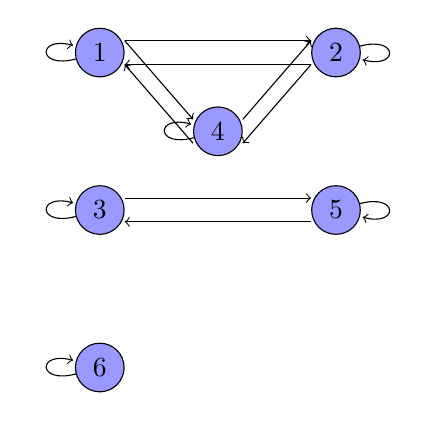
\begin{tikzpicture}


\node[circle, fill=blue!40!white!, draw=black] (1) at (0,0) {1};

\node[circle, fill=blue!40!white!, draw=black] (2) at ($(1) + (3, 0)$) {2};

\node[circle, fill=blue!40!white!, draw=black] (4) at ($(1) + (1.5, -1)$) {4};

\node[circle, fill=blue!40!white!, draw=black] (3) at ($(1) + (0, -2)$) {3};

\node[circle, fill=blue!40!white!, draw=black] (5) at ($(2) + (0, -2)$) {5};

\node[circle, fill=blue!40!white!, draw=black] (6) at ($(1) + (0, -4)$) {6};

\draw[->] ([yshift=1ex]1.east) -- ([yshift=1ex]2.west);
\draw[->] ([yshift=-1ex]2.west) -- ([yshift=-1ex]1.east);

\draw[->] ([yshift=1ex]1.east) -- ([yshift=1ex]4.west);
\draw[->] ([yshift=-1ex]4.west) -- ([yshift=-1ex]1.east);

\draw[->] ([yshift=1ex]4.east) -- ([yshift=1ex]2.west);
\draw[->] ([yshift=-1ex]2.west) -- ([yshift=-1ex]4.east);

\draw[->] ([yshift=1ex]3.east) -- ([yshift=1ex]5.west);
\draw[->] ([yshift=-1ex]5.west) -- ([yshift=-1ex]3.east);

\path (1) edge [loop left] node {} (1);
\path (2) edge [loop right] node {} (2);
\path (3) edge [loop left] node {} (3);
\path (4) edge [loop left] node {} (4);
\path (5) edge [loop right] node {} (5);
\path (6) edge [loop left] node {} (6);

\end{tikzpicture}
\end{center}

\section{Bonus}

\textbf{Solution:} $E \circ F$ is \textbf{NOT} an equivalence relation on A. The composition is $\{(1,1), (1,2), (1,3), (2,1), (2,2), (2,3), (3,2), (3,3)\})$. This is not an equivalence relation because it fails to satisfy the symmetric criteria, missing $\{(3,1)\}$.

Let $A = \{1,2,3\}$. The relation $E = \{(1,1), (2,2), (3,3), (1,2), (2,1)\}$, on $A$. $F = \{(1,1), (2,2), (3,3), (2,3), (3,2)\}$.

In order to calculate the composition, I drew out a digraph, connecting column 1 to column 2, column 2 to column 3.




\end{document}